%%%%%%%%%%%%%%%%%%%%%%%%%%%%%%%%%%%%%%%%%%%%%%%%%%%%%%%%%%%%%%%%%%%%%%%%%%%%%%%%
%                                                                              %
%                    PLANTILLA DE PÓSTER CIENTÍFICO                            %
%                    Formato A0 vertical (portrait)                            %
%                                                                              %
%  Esta plantilla usa la clase a0poster para crear pósters científicos.        %
%  Incluye comandos personalizados para títulos, secciones y texto.            %
%                                                                              %
%%%%%%%%%%%%%%%%%%%%%%%%%%%%%%%%%%%%%%%%%%%%%%%%%%%%%%%%%%%%%%%%%%%%%%%%%%%%%%%%

\documentclass[a0,portrait]{a0poster}

%===============================================================================
%                         PAQUETES NECESARIOS
%===============================================================================
\usepackage[utf8]{inputenc}             % Codificación UTF-8
\usepackage[spanish]{babel}           % Idioma (cambiar a spanish si necesario)
%\usepackage[round]{natbib}              % Citas bibliográficas
\usepackage{graphicx}                   % Imágenes
\usepackage{multicol}                   % Texto en columnas
\usepackage{color}                      % Colores
\usepackage{xcolor}                     % Colores extendidos
\usepackage{colortbl}                   % Colores en tablas
\usepackage{multirow}                   % Celdas multirow en tablas
\usepackage{rotating}                   % Rotar elementos
\usepackage{setspace}                   % Control de interlineado
\usepackage{type1cm}                    % Tamaños de fuente arbitrarios
\usepackage{framed}                     % Cajas con marco
\usepackage{wrapfig}                    % Figuras con texto alrededor
\usepackage{marvosym}                   % Símbolos adicionales

%===============================================================================
%                    IMAGEN DE FONDO (opcional)
%===============================================================================
\usepackage{eso-pic}

% Comando para colocar imagen de fondo centrada
\newcommand\BackgroundPicture{%
    \put(0,0){%
        \parbox[b][\paperheight]{\paperwidth}{%
            \vfill
            \centering
            
\includegraphics[width=\paperwidth,height=\paperheight,%
                keepaspectratio]{esc-ugr-claro}%
            \vfill
        }%
    }%
}
\AddToShipoutPicture{\BackgroundPicture}

%===============================================================================
%                      CONFIGURACIÓN DE COLUMNAS
%===============================================================================
\renewcommand{\columnseprule}{3pt}      % Grosor línea entre columnas
\setlength{\columnsep}{3cm}             % Separación entre columnas
\setlength{\parindent}{3cm}             % Sangría de párrafos
\setlength{\parskip}{.5em}              % Espacio entre párrafos

%===============================================================================
%                       COMANDOS PERSONALIZADOS
%===============================================================================

% --- Título principal del póster ---
% Uso: \titulo{logo}{titulo}{autores}{afiliacion}
%   #1: archivo de imagen del logo (sin extensión)
%   #2: título del póster
%   #3: autores
%   #4: afiliación/institución
\newcommand{\titulo}[4]{%
    \begin{minipage}[c]{10cm}
        \includegraphics[width=10cm]{#1}
    \end{minipage}
    \hfill
    \begin{minipage}[c]{65cm}
        \fontsize{2.2cm}{2.6cm}\selectfont 
        \centering \textbf{\textcolor[rgb]{.5,0,0}{#2}}
        
        \vspace{.5cm}
        
        \begin{center}
            \fontsize{1.8cm}{1.8cm}\selectfont
            \textbf{\textcolor[rgb]{0,0,.5}{#3}}
            
            \vspace{.5cm}
            \fontsize{1.8cm}{1.8cm}\selectfont
            \textbf{\textcolor[rgb]{0,.5,0}{#4}}
        \end{center}
    \end{minipage}
    
    \vspace{1cm}
    \rule{\textwidth}{.2cm}
}

% --- Títulos de sección ---
% Uso: \apartado{Título de la sección}
% Produce texto en mayúsculas, azul, tamaño 45pt
\newcommand{\apartado}[1]{%
    \noindent\fontsize{45pt}{45pt}\selectfont%
    \textcolor[rgb]{0,0,1}{\textbf{\uppercase{#1}}}%
}

% --- Texto normal del póster ---
% Uso: \texto{Contenido del párrafo...}
% Tamaño 30pt, adecuado para lectura a distancia
\newcommand{\texto}[1]{%
    \fontsize{30pt}{30pt}\selectfont #1%
}

% --- Texto pequeño (pies de figura, notas) ---
% Uso: \textochico{Nota o pie de figura...}
% Tamaño 12pt
\newcommand{\textochico}[1]{%
    \fontsize{12pt}{24pt}\selectfont #1%
}

% --- Comando para microlitros ---
\newcommand{\micro}[1]{$#1 \mu l$}

%===============================================================================
%                         DOCUMENTO
%===============================================================================
\begin{document}

% --- Cabecera del póster ---
\titulo{esc-ugr-claro}%
    {Título del Póster: Tema Principal de la Investigación}%
    {Autor1 A, Autor2 B, Autor3 C, Autor4 D}%
    {Departamento. Universidad. Dirección. (email@ejemplo.com)}

% --- Contenido en dos columnas ---
\begin{multicols*}{2}

%-------------------------------------------------------------------------------
\apartado{Introducción}

\texto{
Aquí va el texto de introducción. La vasculogénesis es un proceso que consiste 
en la formación de nuevos vasos sanguíneos a partir de células endoteliales 
diferenciadas de novo.

Incluye el contexto del trabajo, la motivación y los antecedentes relevantes.
Los párrafos deben ser concisos pero informativos, ya que el espacio en un 
póster es limitado.
}

%-------------------------------------------------------------------------------
\apartado{Material y Métodos}

\texto{
Descripción de los materiales y métodos utilizados:

\begin{itemize}
    \item Método 1: descripción breve
    \item Método 2: descripción breve
    \item Análisis estadístico utilizado
\end{itemize}
}

%-------------------------------------------------------------------------------
\apartado{Resultados}

\texto{
Presentación de los resultados principales.
}

% --- Ejemplo de figura con pie ---
\begin{center}
\begin{minipage}[t]{\columnwidth}
    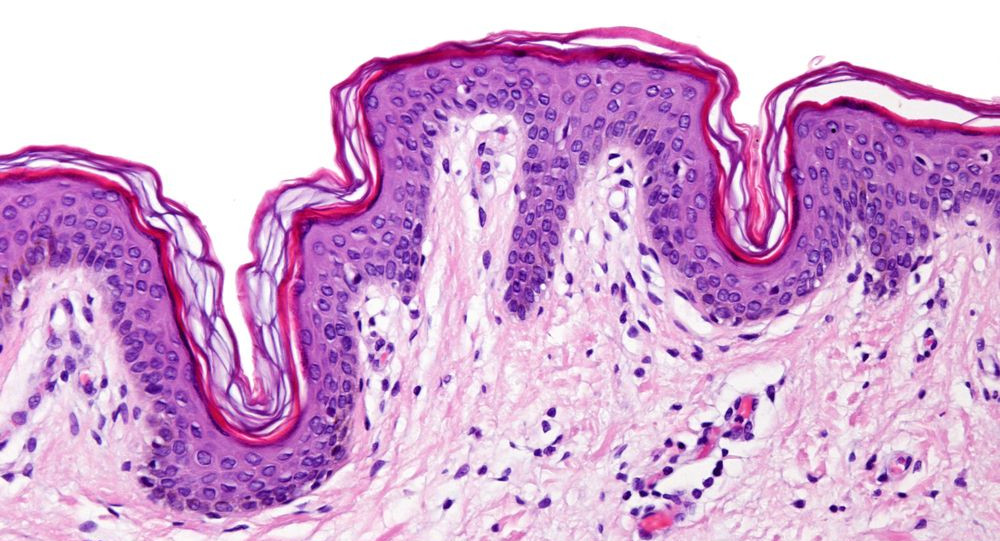
\includegraphics[width=\textwidth]{fotos/Fig1poster}
    
    \begin{framed}
        Fig. 1. Descripción detallada de la figura. Incluir información 
        relevante sobre lo que muestra la imagen, las condiciones experimentales 
        y la escala si es aplicable.
    \end{framed}
\end{minipage}


\vfill

\begin{minipage}[t]{0.55\columnwidth}
Praesent vitae porttitor tortor. Fusce mollis, lacus ut ullamcorper molestie, justo ligula congue velit, ut maximus magna lorem vitae arcu. Sed sodales justo nec faucibus ultricies. Nam dictum enim non venenatis egestas.
\end{minipage}
\end{center}

\begin{center}
	\begin{minipage}[t]{0.4\columnwidth}
		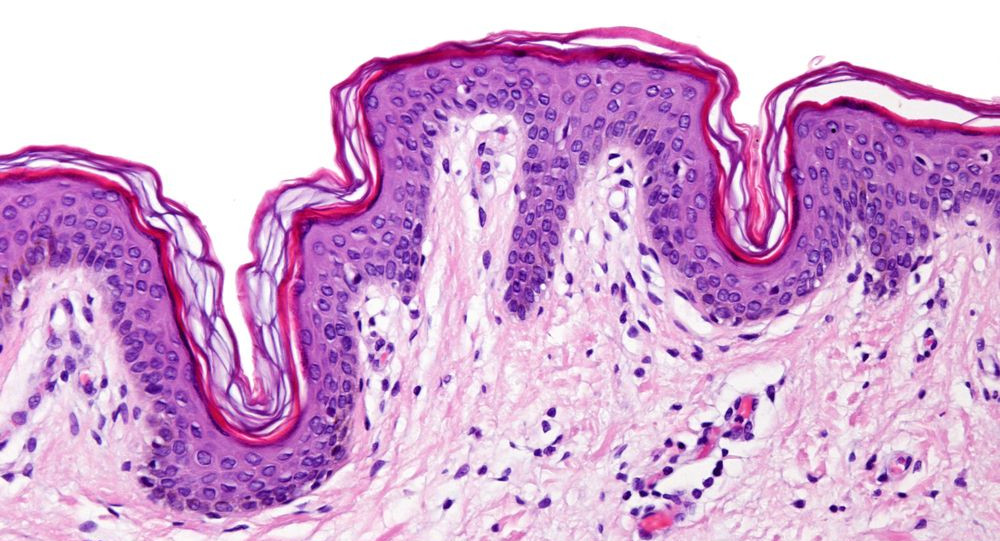
\includegraphics[width=\textwidth]{fotos/Fig1poster}
		
		\begin{framed}
			Fig. 1. Descripción detallada de la figura. Incluir información 
			relevante sobre lo que muestra la imagen, las condiciones experimentales 
			y la escala si es aplicable.
		\end{framed}
	\end{minipage}
\end{center}

\begin{center}
	\begin{minipage}[t]{\columnwidth}
		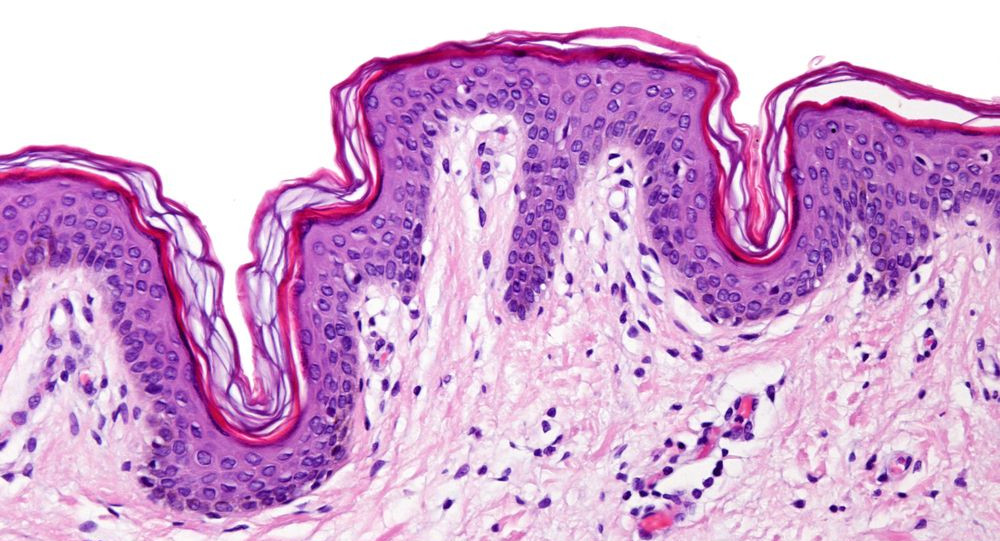
\includegraphics[width=\textwidth]{fotos/Fig1poster}
		
		\begin{framed}
			Fig. 1. Descripción detallada de la figura. Incluir información 
			relevante sobre lo que muestra la imagen, las condiciones experimentales 
			y la escala si es aplicable.
		\end{framed}
	\end{minipage}
\end{center}

\texto{
	Praesent vitae porttitor tortor. Fusce mollis, lacus ut ullamcorper molestie, justo ligula congue velit, ut maximus magna lorem vitae arcu. Sed sodales justo nec faucibus ultricies. Nam dictum enim non venenatis egestas. Fusce ut nisl in magna lobortis posuere nec a nunc. Cras luctus sit amet augue in imperdiet. Nulla facilisis tristique velit, eget auctor tellus suscipit quis. Fusce tincidunt a leo sit amet aliquam. Vestibulum ante ipsum primis in faucibus orci luctus et ultrices posuere cubilia curae; Sed suscipit dignissim facilisis. Etiam ut erat quis turpis tincidunt accumsan vitae non magna. Etiam non metus sapien. Phasellus suscipit libero eu neque dignissim, non dignissim magna lacinia.
}

%-------------------------------------------------------------------------------
\apartado{Discusión}

\noindent
Interpretación de los resultados en el contexto de la literatura existente. 
Comparación con estudios previos y explicación de posibles discrepancias.

Praesent vitae porttitor tortor. Fusce mollis, lacus ut ullamcorper molestie, justo ligula congue velit, ut maximus magna lorem vitae arcu. Sed sodales justo nec faucibus ultricies. Nam dictum enim non venenatis egestas. Fusce ut nisl in magna lobortis posuere nec a nunc. Cras luctus sit amet augue in imperdiet. Nulla facilisis tristique velit, eget auctor tellus suscipit quis. Fusce tincidunt a leo sit amet aliquam. Vestibulum ante ipsum primis in faucibus orci luctus et ultrices posuere cubilia curae; Sed suscipit dignissim facilisis. Etiam ut erat quis turpis tincidunt accumsan vitae non magna. Etiam non metus sapien. Phasellus suscipit libero eu neque dignissim, non dignissim magna lacinia.

\begin{minipage}{\textwidth}
	contenidos...
\end{minipage}

Praesent vitae porttitor tortor. Fusce mollis, lacus ut ullamcorper molestie, justo ligula congue velit, ut maximus magna lorem vitae arcu. Sed sodales justo nec faucibus ultricies. Nam dictum enim non venenatis egestas. Fusce ut nisl in magna lobortis posuere nec a nunc. Cras luctus sit amet augue in imperdiet. Nulla facilisis tristique velit, eget auctor tellus suscipit quis. Fusce tincidunt a leo sit amet aliquam. Vestibulum ante ipsum primis in faucibus orci luctus et ultrices posuere cubilia curae; Sed suscipit dignissim facilisis. Etiam ut erat quis turpis tincidunt accumsan vitae non magna. Etiam non metus sapien. Phasellus suscipit libero eu neque dignissim, non dignissim magna lacinia.

%-------------------------------------------------------------------------------
\apartado{Conclusiones}

\texto{
\begin{enumerate}
    \item Primera conclusión principal
    \item Segunda conclusión principal
    \item Implicaciones del trabajo
\end{enumerate}
}

%-------------------------------------------------------------------------------
\apartado{Bibliografía}

\textochico{
1. Autor A, et al. (2020). Título del artículo. Revista 10:100-110.\\
2. Autor B, et al. (2019). Título del artículo. Revista 5:50-60.\\
3. Autor C, et al. (2018). Título del artículo. Revista 8:80-90.
}

%-------------------------------------------------------------------------------
\apartado{Agradecimientos}

\textochico{
Este trabajo ha sido financiado por... 
Agradecemos a... por su colaboración.
}

\end{multicols*}
\end{document}
